	\chapter{Detecting \ac{EWFO} on \ac{MAV}}
	\label{sec:object_detection}
	
	\acp{EWFO} differ from solid texture rich objects as their features are sparse and spread over large parts of the image. The m
	\ac{CNN}-based Object Detectors offer the advantage that they can be trained on any object given labelled training data is available. However, typically the architectures of \acp{CNN} are optimized for solid feature rich objects, such as planes, cars or faces. The predominant metrics optimized are precision and recall rather than inference speed. This work investigates the detection of \ac{EWFO} on \acp{MAV} as part of a control loop. Hence, inference speed and computational requirements can be more important than detection performance. Furthermore, \acp{EWFO} differ substantially from objects usually used in Object Detection. This chapter investigates the detection of \acp{EWFO} with a \acp{CNN}. An off-the-shelve \acp{CNN}-based detector is optimized for the detection of \acp{EWFO}. Furthermore, the trade-off in detection performance and inference speed is studied in the example of the hardware used in this thesis. The research questions are summarized in the following:
	
\begin{enumerate}
	\item[\textbf{RQ2}]How can a \acp{CNN} be used to detect \acp{EWFO} efficiently?
	
\end{enumerate}

	\section{Methodology}
		
	This work uses a typical one-stage detector with anchor boxes as baseline, namely the \textit{YoloV3} detector with the \textit{TinyYoloV3} network. The fundamental concept of one-stage detectors with anchor boxes is illustrated in \Cref{sec:related}. In this section the implementation with the \textit{TinyYoloV3} network and its training goal are explained.
	
	On a high level basis \textit{YoloV3} maps the input image to a predefined set of anchor boxes which are visualized in \Cref{sec:anchors}. The anchors have a predefined width $p_w$, height $p_h$ and are arranged in grids corresponding to the spatial resolution of the output layers. For objects of different scales different image features are relevant. Furthermore, for small objects a more fine grain resolution is required to sufficiently distinguish between multiple small objects close to each other. Therefore, \textit{YoloV3} uses two output grids $G=2$ output grids, with a grid of $S_1 =13$ for larger objects (red) and $S_2 = 26$ smaller objects (blue). 
	
	For each box the network predicts an object probability $\hat o$ that classifies the class as object (1) or background (0). The original version of \textit{YoloV3} further distinguishes between object classes, however this work considers the single class case. There we remove this output node from the prediction. 
	
	The predefined anchors only cover a subset of possible areas that can contain an object. Hence, \textit{YoloV3} also predicts how to adapt the anchor box to better fit the predicted object. These are  the bounding box center $b_x,b_y$ as well as its width $b_w$ and height $b_h$. 
		
	In total this leads to 5 predicted parameters for each bounding box and thus to a mapping from the input image of 416x416x3 pixels to 12675 output nodes that predict 2535 boxes. In a last step boxes that contain the same class and have a high overlap are filtered such that only the boxes with the highest confidences remain.	
			
	This mapping is implemented with a \acp{CNN} as illustrated in  \Cref{fig:tinyyolov3_arch}. It contains 10 convolutional, 6 pooling and 1 unpooling layer(s). After each convolutional layer batch normalization normalizes the output in order to simplify the training process.
	The input image with a resolution of 416x416x3 is processed by 5 layers that stepwise decrease the spatial resolution (max pooling) while increasing the width, leading to a intermediate volume of 26x26x512. This part can be seen as a common part that extracts features for objects at all scales. The architecture is a typical example of current \acp{CNN}. In the early layers the receptive field of the filters is small. Hence, the patterns that can be represented are not very complex and only a small amount of filters is used. As the network gets deeper more complex patterns can be present and more weights are required to encode these features. Hence, the width is increased. Research has shown that fixing kernels to a size of 3x3 and stacking them in deep layers is particularly efficient\todoref{vgg}. This can also be seen in the \textit{TinyYoloV3} architecture. 
	
	Convolving the wide volume of deeper layers such as the 26x26x512  output of layer 5 with a 3x3 kernel requires many computations. Therefore a common technique is to first compress the volume by applying a 1x1 kernel intermediately. Such \textit{bottleneck} layers can be seen in layer 6-1 and 7-2.
	
	From layer 5 the network splits to two branches responsible for smaller and larger objects. The lower branch extracts features for larger objects leading to a final grid of 13x13. The higher branch extracts features for smaller objects leading to a grid of 26x26. When Although not stated explicitly by the authors this is likely to compress the feature response of the previous layer and thus save computations.
	
	In the final layer 15 output nodes are responsible to predict 3 bounding boxes for each grid cell. Thereby the nodes responsible for $\hat o$ have a sigmoid-activation such that the response gets squashed between 0 and 1 thus can be interpreted as a probability. Similarly the nodes responsible for $\hat x$ and $\hat y$ have a sigmoid activation such that the output can be interpreted as coordinate normalized to the image size. For the output nodes of $w$ and $h$ \textit{YoloV3} uses $e^x$-activation. This way the output is always larger than one while no adaption in bounding box width/height ($w=1$) corresponds to no activation. Furthermore, the network can predict a large range of scales in a small range of activation which aims to simplify the learning process.
	
			
	\begin{figure}[hbtp]
		\centering
		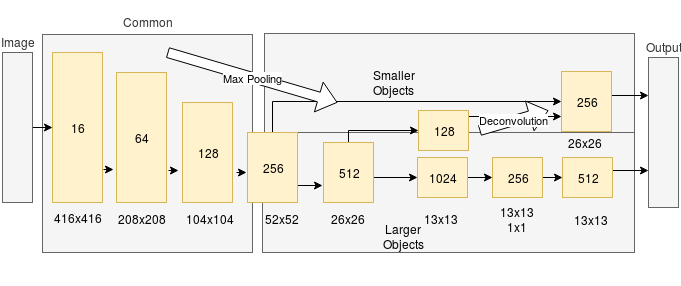
\includegraphics[width=0.8\textwidth]{fig/tinyyolov3_arch}
		\caption{The architecture of the baseline \textit{TinyYoloV3}. For each layer the amount of filters are displayed. The height of the boxes correspond to their spatial dimension. Arrows correspond to the forward pass in a network inference. In the common part the spatial resolution decreases each layer down to 26x26, while the width increases from 16 to 512. From layer 5 two branches focus on objects corresponding to different scales. }
		\label{fig:tinyyolov3_arch}
	\end{figure}
	

	\subsection{Training Goal}
	
	In order to train a \ac{CNN} to predict the desired properties a ground truth has to be defined for each of the 12675 output nodes. Subsequently the loss is formulated as derivable function and the \ac{CNN} can be trained with backpropagation.
	
	Thereby it is desirable that a network output of zero corresponds to no network activation and henceforth to keep all predicted bounding boxes in the default shape. Therefore, \textit{YoloV3} encodes the ground true coordinates as follows:
	 
	
	\begin{equation}
	\label{sec:encoding}
	b_x = \sigma(\hat x_{i,j,k}) + g^x_{i,j}\quad
	b_y = \sigma(\hat y_{i,j,k}) + g^y_{i,j}\quad
	b_w = e^{\hat w_{i,j,k}} \cdot p^w_{i,j,k}\quad
	b_h = e^{\hat h_{i,j,k}} \cdot p^h_{i,j,k}
	\end{equation}
	
	where $\hat{x}$,$\hat{y}$,$\hat w_{i,j,k}$ and $\hat h_{i,j,k}$ correspond to output nodes of anchor box at grid $i$, cell $j$, anchor $k$; $g^x_{i,j,k}$, $g^y_{i,j}$ is the top left coordinate of the respective grid cell; $\sigma$ is the sigmoid-function.
	
	The question remains to which grid cell and anchor box a label is assigned to. Therefore the \ac{IoU} between every ground truth and anchor box is calculated and the grid with the highest value is assigned. If a ground truth box has very different coordinates than any possible anchor box, even the highest \ac{IoU} is comparatively low. Thus the network has to perform a very strong activation to predict such a label. In return the gradient will be high which can cause unstable updates. Therefore labels that have a lower \ac{IoU} than 0.5 are excluded. 
	
	With the true label and the predicted label the training goal can be formulated. The loss needs to capture the localization and the classification goal. In a typical ground truth image only a small subset of anchors is assigned responsible to predict an object. All the other anchors see only background. Hence, there is a class imbalance between the "object" class and the "background" class. Treating both losses equally would lead the model to simply assign "background" for all anchors. The weight terms $\lambda_{obj}$ and $\lambda_{noobj}$ compensate for this class imbalance. Furthermore, $\lambda_{loc}$ trades-off the localization goal and the classification goal. The abstract training loss is summarized in: 

	\begin{equation}
	\mathcal{L} = \lambda_{loc}\mathcal{L}_{loc} + \lambda_{obj}\mathcal{L}_{obj} + \lambda_{noobj}\mathcal{L}_{noobj} + \lambda_{class}\mathcal{L}_{class}
	\end{equation}
	where $\mathcal{L}_{loc}$ is the loss for bounding box dimensions, $\mathcal{L}_{obj}$ the loss where a object is present, $\mathcal{L}_{noobj}$ the loss where there is no object. The weights are kept to the default value of $\lambda_{loc} = 5$,$\lambda_{obj} = 5$ and $\lambda_{noobj} = 0.5$.
	
	The object loss quantifies a binary classification loss. Hence, it is the difference between a predicted probability $\hat o$ and an actual class label $c$. Where $o \in \{0,1\}$ and $\hat o \in (0,1)$. In order to learn such a goal it is desirable that the weights of the network get updated significantly when the difference between truth and prediction are high. However, when prediction and truth are already close to each other, the updates to the weights should be smaller otherwise the training might miss the optimal solution. A loss function that contains the desired properties and is used by \textit{YoloV3} is the logarithmic loss which can be formulated as follows:
	
	\begin{equation}
		\mathcal{L}_{log} = -(o_{ij}\log(\hat o_{ijk}) + (1 - o_{ij})\log(1 - \hat o_{ijk}))
	\end{equation}
	
	where $\hat o_{ij}$ is an output node with sigmoid activation assigned to anchor box $i$,$j$,$k$ and $ o_{ij}$ the ground truth label assigned to that box. The logarithmic loss is calculated for each output grid $G_i$, for each grid cell $S_j$ and each anchor box $B_k$. However, only the loss of the responsible anchor boxes are summed in the total loss calculation:
	
	\begin{equation}
		\mathcal{L}_{obj} = \sum_{i=0}^{G}\sum_{j=0}^{S_i^2}\sum_{k=0}^{B_i} \mathbb{1}_{ijk}^{obj}(-(c_{ijk}\log(\hat c_{ijk}) + (1 - c_{ijk})\log(1 - \hat c_{ijk})))
	\end{equation}
	
	Thereby the  binary variable $\mathbb{1}_{ijk}^{obj}$ is 1 if an object is present at anchor $i,j,k$. $\mathcal{L}_{obj}$ is defined vice versa but controlled by the $\mathbb{1}_{ijk}^{noobj}$ binary variable.

	For the localization loss, similar to the classification loss, the weights should be updated significantly when the difference is high but less strongly when the difference is small. Furthermore, the loss should be invariant to direction. A loss that contains these properties is the squared distance between each bounding box parameter. However, the squared distance does not make a difference between large and small boxes. For example, a deviation of 5 px for a small ground truth box with a width of 1 is treated equally to a deviation from a ground truth box with width 100. Therefore \textit{YoloV3}, applies the square root on width and height to scale down very large box dimensions and thus balance the loss calculation. The localization loss is summarized in:
	
	\begin{equation}
		\mathcal{L}_{loc} = \sum_{i=0}^{G} \sum_{j=0}^{S_i^2}\sum_{k=0}^{B_i} \mathbb{1}_{ijk}^{obj}[(x_{ijk}-\hat{x}_{ijk})^2 + (y_{ijk}-\hat{y}_{ijk})^2  + (\sqrt{w_{ijk}}-\sqrt{\hat{w}_{ijk}})^2 +(\sqrt{h_{ijk}}-\sqrt{\hat{h}_{ijk}})^2 ]
	\end{equation}
	where $x_{ijk}$,$y_{ijk}$ are the ground truth center coordinates of anchor box $i,j,k$ and $w_{ijk}$,$h_{ijk}$ the corresponding width and height. $\hat x_{ijk}$,$\hat y_{ijk}, \hat w_{ijk}$,$\hat h_{ijk}$ are the predicted bounding box coordinates. 
	
	The model is implemented using \textit{keras} with \textit{tensorflow} backend. 
	
	\subsection{Datasets}
	
	Throughout the experiments the same training and test set is used. For training 20 000 samples from the dataset created in \Cref{sec:datagen} are used. For testing we use the test set described in \Cref{sec:datagen:method}.

	For all trainings the Adam optimizer is applied using a learning rate of 0.001 for the first 60 epochs and a learning rate 0.0001 afterwards. A validation set containing 1\% randomly sampled images from the training set is used. The training is stopped if the validation error does not decrease for more than 5 epochs or 100 epochs are reached.
	
		\section{Refining the architecture}
	
	\textit{TinyYoloV3} is optimized to detect solid feature rich objects of multiple classes with a low computational budget. This led to an architecture with 9 layers and a final width of 1024. Thereby the receptive field is of the last layer is 223 pixels. For solid objects this is of minor impact as even if the network only sees an object part it can still learn to recognize it. However, this does not apply for \acp{EWFO} which are empty and do not contain any information in the object centre. Instead it can confuse an output layer that is assigned responsible to detect such an object. We hypothesize that a larger receptive field will benefit the performance for objects of higher scale. Furthermore, \acp{EWFO} consist only of simple features. Hence we hypothesize that less filters are required to represent such an object and a thinner model can perform equally well than its wider counterpart. Finally, \acp{EWFO} are not very complex. Hence, we hypothesize that a shallower model should be able to learn the task equally well.
	
	The anchor box concept introduces additional hyperparameters. By choosing the anchor box dimensions close to objects that appear in training/test set prior knowledge can be included. The better the anchor boxes fit the appearing object the less work has to be done by the network and hence performance can potentially be improved. Hence, we evaluate whether redesigned anchor boxes improve the network performance. 
	
	\begin{figure}[hbtp]
		\centering
		\begin{minipage}{0.3\textwidth}
			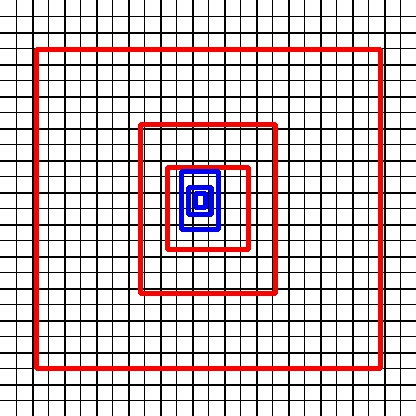
\includegraphics[width=\textwidth]{fig/yolov3_anchors}
		\end{minipage}
		\begin{minipage}{0.3\textwidth}
			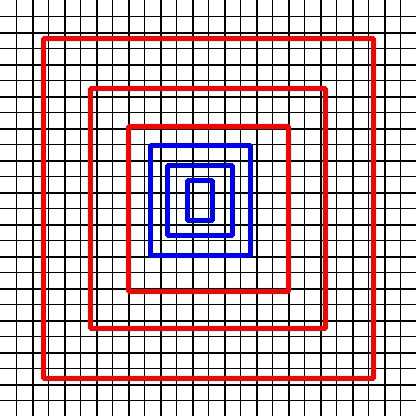
\includegraphics[width=\textwidth]{fig/gate_anchors}
		\end{minipage}
		\caption{ Visualization of the anchor parametrization. It can be seen the two output grids, where the grid for larger scale objects is drawn thicker. For both output grids the anchor at the center location is displayed. The anchor for smaller objects in blue, the anchors for larger objects in red. The left image shows the baseline \textit{TinyYoloV3} anchors. The right image the anchors based on a k-means clustering of the training set. }
		\label{fig:anchors}
	\end{figure}
	
	\subsection{Experiments}
	
	Initially an architecture evaluation is performed. Therefore different architectures are trained and evaluated in terms of \ac{ap60}. As an architecture contains many parameters we can not simply vary each of them independently. Hence, three experiments are performed iteratively. We first describe them on a high level basis before explaining the exact changes. In a first step the width is decreased until a drop in performance is noticeable. In a second step the architecture with the lowest width but without performance drop is chosen and the depth is varied. Based on the results of this step we create a final model that combines the gained insights and tune the anchor boxes.
	
	The scheme in which the architecture is changed is visualized in \Cref{fig:depth_changes}. The width of the baseline model is decreased stepwise by a factor of two. When decreasing depth only convolutional layers are removed while the pooling layers are kept such that the spatial resolution stays the same. When increasing depth 2 layers are inserted stepwise at the end of both branches. The results show how depth is mainly relevant to detect objects of larger scale. Hence, the final model consist of 5 common layers, 15 layers on the branch to detect larger objects and 2 layers on the branch to detect small objects.
	
	
	\begin{figure}[hbtp]
		\centering
		\includegraphics[width=0.9\textwidth]{fig/depth_changes}
		\caption{Architectural Changes when varying the depth. The upper graph shows in which order layers are removed. The lower graph shows how layers are added. Depth is increased by inserting two layers on each branch (green). }
		\label{fig:depth_changes}
	\end{figure}
	
	
	
	\subsection{Results}
	
	\Cref{fig:perf_width} shows the performance for thinner and wider networks. It is apparent how the performance only undergoes slight variations despite reducing the total number of weights by a factor 1000. \todo{retrain one in the middle to get variance, it should be more linear}
	
	
	\begin{figure}[hbtp]
		\centering
		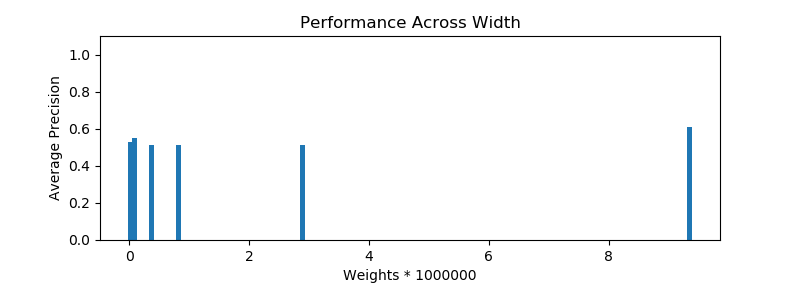
\includegraphics[width=\textwidth]{fig/perf_width}
		\caption{Performance in simulation when varying the amount of filters per layer. Starting from the baseline architecture with approximately 9 Mio. weights, the amount of filters per layer are decreased stepwise by a factor of 2. Only minor effects on performance can be seen, despite reducing the flexibility of the model.}
		\label{fig:perf_width}
	\end{figure}
	
	\begin{figure}[hbtp]
		\centering
		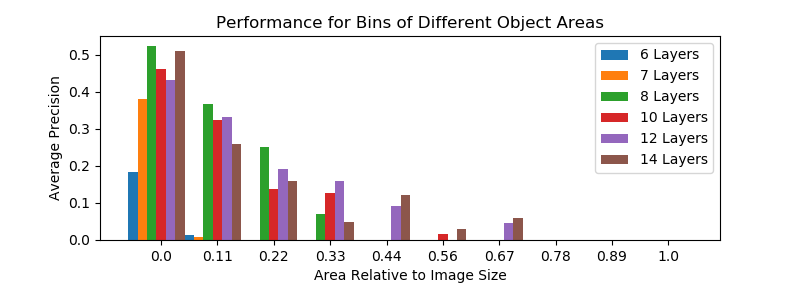
\includegraphics[width=\textwidth]{fig/depth_ap_size}
		\caption{Performance in simulation of models with varying depth and for bins of different size. It can be seen that the performance for larger objects increases with the amount of layers.}
		\label{fig:depth_ap_size}
	\end{figure}
	
	\Cref{fig:size_bins} shows the distribution of object sizes in the bins used for evaluation. It can be seen that most objects in the test set are further away. \todo{put some examples to show what each size actuall means}
	
	\begin{figure}[hbtp]
		\centering
		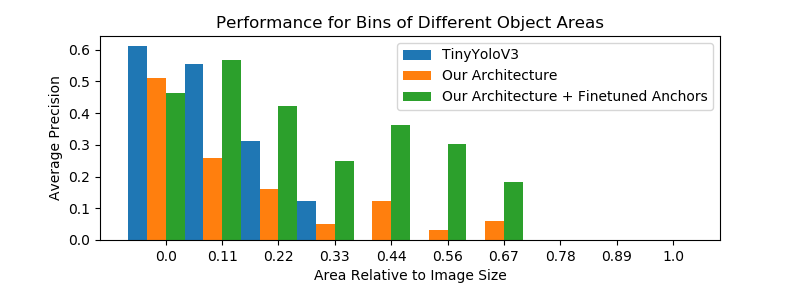
\includegraphics[width=0.8\textwidth]{fig/hyperparam_size}
		\caption{Architectural Changes when varying the depth. The upper graph shows in which order layers are removed. The lower graph shows how layers are added. Depth is increased by inserting two layers on each branch (green). }
		\label{fig:hyp}
	\end{figure}
	
	\begin{figure}[hbtp]
		\centering
		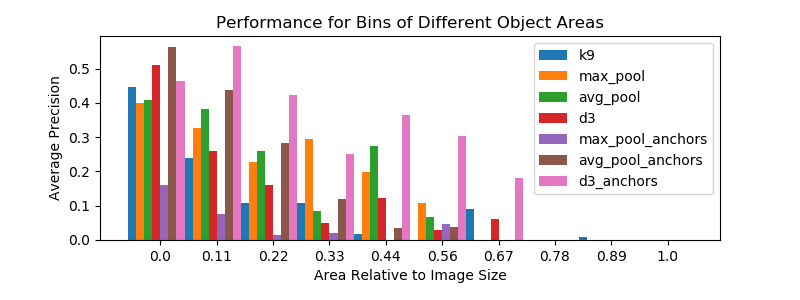
\includegraphics[width=\textwidth]{fig/rf_ap_size}
		\caption{Label distribution in bins of different object size. As the field of view is larger for objects further away, the proportion of small objects is higher.}
		\label{fig:size_bins}
	\end{figure}
	
	\subsection{Discussion}
	
	The overall performance is only slightly affected when reducing the number of weights in terms of width and height. We can assume that this is because the objects we investigate are of quite simple structure. Intuitively the features to be considered are color, lines and edges in certain combinations. Hence, it seems logical that only a few filters are necessary to represent these shapes.
	
	The performance in terms of different object sizes varies significantly for models with varying depth. Only deeper networks are able to detect larger objects. However, the complexity of the object does not increase for closer objects. In contrary the closer the objects are, the less context is visible. A very close object consists "only" of an orange square. Hence, it is unlikely that increased flexibility is the reason for the increase in performance. 
	
	Instead it is more likely that the increased receptive field is the reason for the improved performance. In fact only the network with 14 layers has a receptive field of 414 an thus covers the whole image. Yet even this network cannot detect the largest objects. Thus the receptive field can not be the only reason for the lower performance on larger objects.
	
	The current structure combines features distributed across space in a pyramid fashion. So 3-by-3 convolutions are performed layer by layer such until the whole image is covered. For \acp{EWFO} many of these steps are unnecessary as the objects are empty and the network should learn to ignore the empty part in the centre. It is possible that this structure gets confused by the parts that are present in the image centre.
	
	\subsection{Conclusion}
	
	We investigated how width affects the performance for the detection of \acp{EWFO}. We hypothesized that due to the low variance in the investigated object and the simple features, less filters are required than in the baseline architecture. We can confirm this hypothesis as we see that the width can be decreased by a factor of 10 without loosing performance. This leads to a reduction of weights by a factor of 1000. 
	
	Furthermore, we investigated how depth affects the performance of the model. We hypothesized that a shallow network should be able to detect the object as it only consists of relatively simple features. We can see how depth is required in order to cover the whole input image. Hence, we cannot fully conclude whether depth is required for the increased flexibility or simply due to the receptive field. 
	
	
	\section{Detecting Empty Objects}
	
	As could be seen in \Cref{sec:methodology}, \textit{TinyYoloV3} similar to most current \acp{CNN} combine simple features to a more abstract representation layer by layer. Thereby pooling reduces task irrelevant information and reduces the spatial dimension. At the same time the number of filters is increased to encode the more complex patterns. in the deeper layers more and more area of the image is covered. In the final layer each location in the volume encodes the patterns that are present in the respective field of the preceding filters and an object prediction is performed.
	
	In \acp{EWFO} the largest part of the object is empty while the actual features are simple edges and corners. Hence, the filters should activate on these simple features while ignoring the empty part. However, the empty part can contain any kind of object and thus activate the network. Whether the information does not belong to an object can only be decided when information about the object border is present in the receptive field of the filter. Hence, we hypothesize that despite the relatively simple shape of \acp{EWFO} their detection with \acp{CNN} is not an easy task.
	
	If our assumption is correct, the detection should get worse as the features are spread more apart. Hence, the performance should decrease as the object gets closer. This would be the opposite for typical solid objects. For example \todoref{object detect tensorflow} report an increase in detection performance with object size on the common Object Detection benchmarks. On the other hand \ac{EWFO} also have thin structures. Therefore, the performance should also decrease for very small objects.
	
	Furthermore, if emptiness is really the reason for a decrease in performance, covering the empty part with a certain pattern should lead to the opposite result. In this case the detector could exploit the information present in the solid part and would not be distracted by background or other objects.
	
	\subsection{Experiment}
	
	A dataset is created in which the empty part is augmented with a distinctive pattern. An example can be seen in \Cref{fig:cats}. For training 20 000 samples are created and a network is trained. For testing a test set with 150 samples is created. The view points are limited to frontal views. 
	
	On this dataset three models are tested: Model I, the baseline TinyYoloV3 architecture , Model II our refined architecture, Model III the refined architecture trained when the object is augmented with the distinctive pattern.
	
		\begin{figure}
		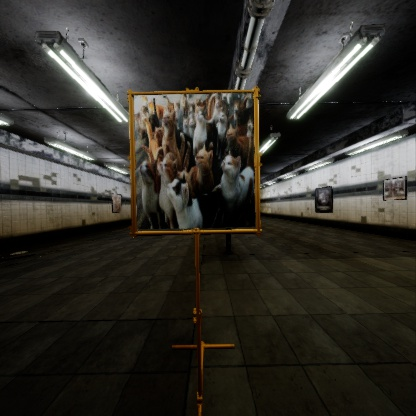
\includegraphics[width=\textwidth]{fig/cats}
		\caption{An example of the augmented object. A \acp{CNN} can exploit this structure and should be less distracted by background.}
		\label{fig:cats}
	\end{figure}
	
	\subsection{Results}

	\subsection{Discussion}
	
	\subsection{Conclusion}
	
	
